\documentclass[11pt,a4paper]{letter}
\usepackage[utf8]{inputenc}
\usepackage[spanish]{babel}
\usepackage{hyperref}
\usepackage{pdfpages}

\signature{Prof. César Rodríguez \\ Laboratorio de Electrónica y Computación \\ Universidad de Oriente \\ Núcleo de Sucre, Venezuela}
\address{Universidad de Oriente, Venezuela \\ Núcleo de Sucre \\ Escuela de Ciencias \\ Dpto. de Física \\ cel: (0412) 1883184) \\ email: cero2k6@gmail.com}

\begin{document}

\begin{letter}{<Nombre del Inversor o Empresa Destinataria> \\ <Cargo del Inversor> \\ <Dirección de la Empresa>}

\opening{Estimado/a <Nombre del Inversor>,}

Me dirijo a usted para presentarle una oportunidad de inversión estratégica basada en el documento 'Private AI Lab Blueprint'. El objetivo de esta solicitud es buscar su respaldo económico para la creación de un Laboratorio de Inteligencia Artificial 100\% local, diseñado específicamente para proveer herramientas de IA a organizaciones e instituciones como la suya de forma segura, privada y altamente eficiente.

Actualmente, la adopción corporativa de la inteligencia artificial depende casi exclusivamente de servicios en la nube, lo cual implica enviar información sensible a servidores de terceros donde se desconoce qué harán exactamente con esos datos. Nuestro laboratorio propone un paradigma basado en la \textbf{soberanía digital}, asegurando que su empresa tenga el control absoluto para decidir cómo y cuándo utilizar la inteligencia artificial. De esta manera, garantizamos la privacidad total de sus operaciones y evitamos que sus datos confidenciales terminen siendo utilizados para la inserción de anuncios o tácticas de monetización de grandes plataformas.

Además de la seguridad, el control de costes es una ventaja fundamental. Delegar las operaciones de su organización a modelos en la nube genera un alto coste económico continuo. Esto se vuelve especialmente peligroso al implementar agentes autónomos; tener múltiples agentes iterando por su cuenta en la nube puede resultar en un descontrol financiero que genere facturas altísimas a final de mes. Recientemente, los grandes proveedores han comenzado a ser conscientes de los altos costos de mantenimiento, lo que inevitablemente llevará a una subida generalizada de precios. Al invertir en este laboratorio local, eliminamos el pago recurrente por el consumo de tokens y protegemos el presupuesto de su organización.

El entorno técnico que proponemos está basado en los estándares de seguridad más exigentes. No instalaremos herramientas de IA directamente en los sistemas para evitar inestabilidades o vulnerabilidades, sino que desplegaremos toda la infraestructura en contenedores aislados y sin privilegios de administrador (modo Rootless), mitigando el riesgo de que la IA pueda tomar control indebido del sistema. 

A nivel operativo, proporcionaremos a sus equipos interfaces amigables e intuitivas idénticas a las grandes soluciones comerciales, pero que usted podrá autoalojar de forma local. Mediante el desarrollo de sistemas RAG (Retrieval-Augmented Generation) programados a medida en lenguajes como Python o Rust, construiremos una 'memoria digital' o 'cerebro propio' que procesará todos los documentos y la base de conocimiento interno de su entidad. Esto permitirá a sus profesionales realizar búsquedas complejas, programar scripts y extraer información crítica de forma inmediata, procesando todo localmente en sus propias tarjetas gráficas y sin que un solo byte de información escape hacia internet.

Para ilustrar el impacto real que esta tecnología puede tener en infraestructuras críticas del Estado, hemos desarrollado un caso de uso práctico enfocado en la optimización del \textbf{Sistema Hídrico de Cumaná}. Le invito a revisar los detalles de esta propuesta en el anexo incluido al final de este documento.

Estoy convencido de que la implementación del 'Private AI Lab Blueprint' no solo resguardará los datos más sensibles de su institución, sino que multiplicará exponencialmente la productividad de sus equipos mediante herramientas inteligentes y adaptadas a sus necesidades operativas.

Me encantaría agendar una reunión para mostrarle en detalle la presentación de nuestra arquitectura y discutir cómo esta inversión inicial se traducirá en ahorros sostenidos y seguridad para su infraestructura.

\closing{Atentamente,}

\end{letter}
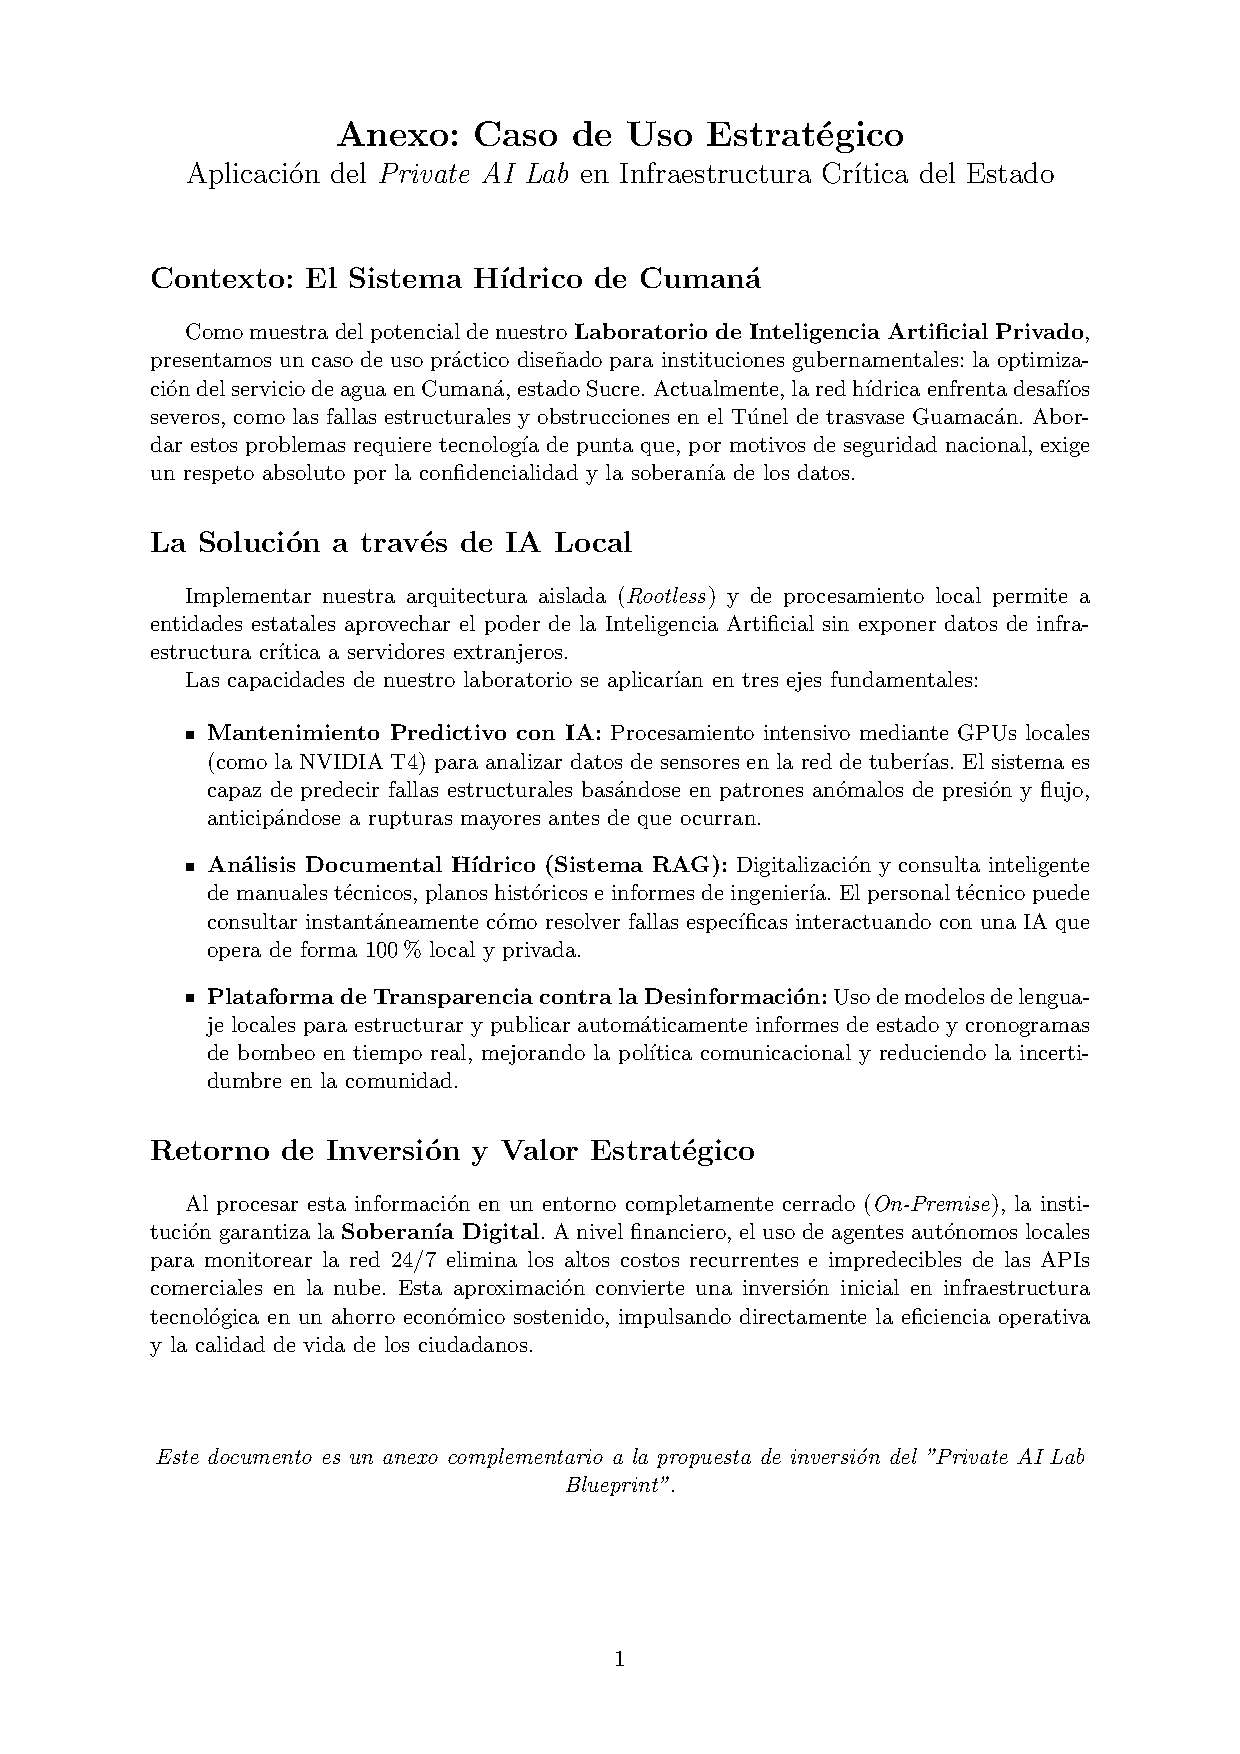
\includepdf[pages=-]{anexo_caso_uso_cumana.pdf}
\end{document}